%!TEX program = xelatex
\documentclass{standalone}
\usepackage{tikz}
\usepackage{tikz-qtree}
\usepackage{xcolor}
\usetikzlibrary{arrows}
\usepackage{fontspec}
\setmainfont{Helvetica}
\begin{document}
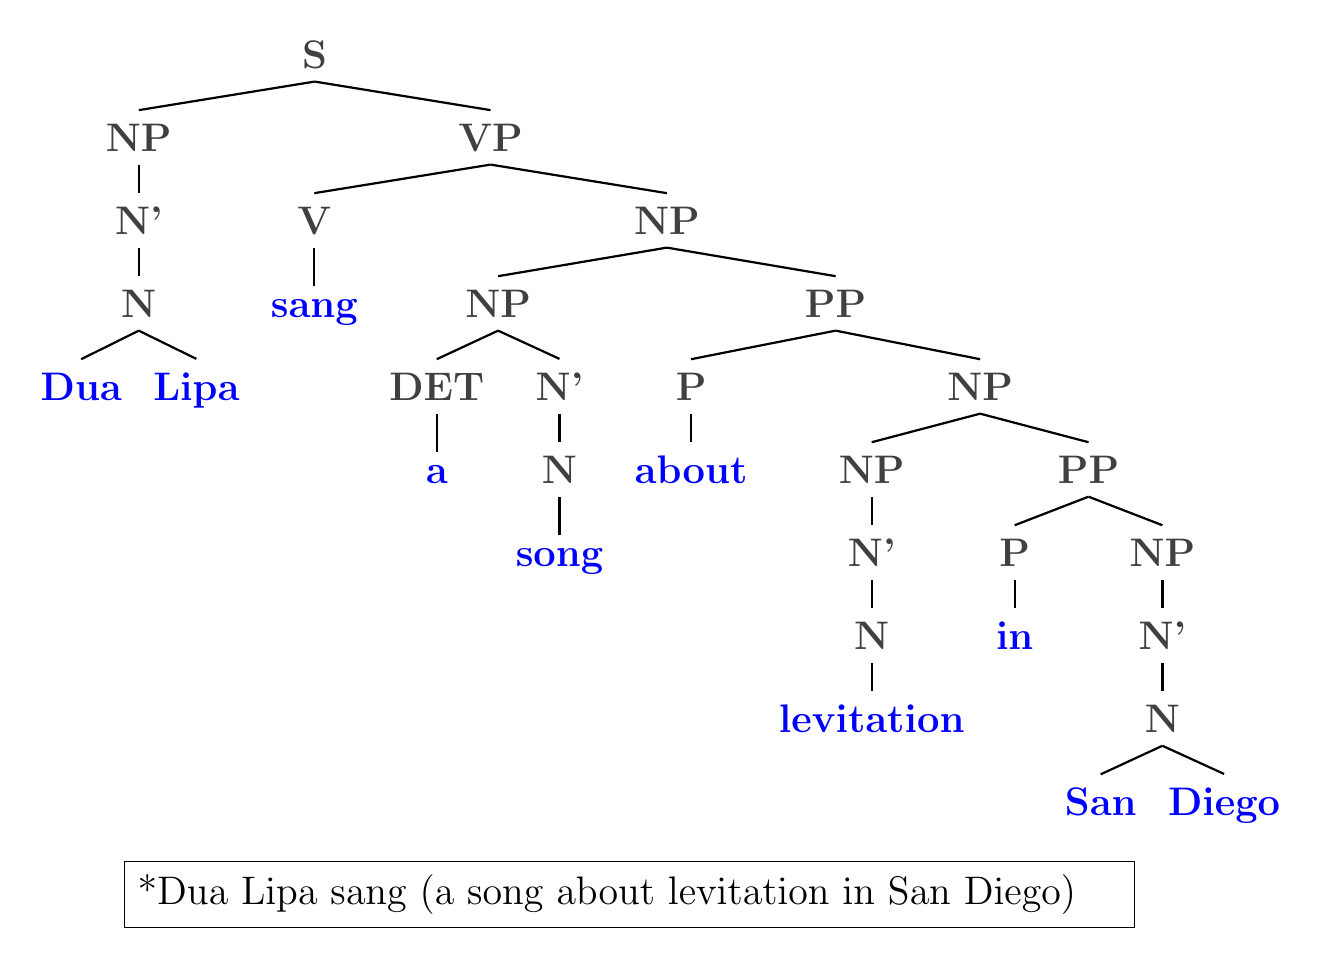
\begin{tikzpicture}
\tikzset{level distance=30pt}
\tikzset{every  leaf node/.style={text=blue,font=\bf}}
\tikzset{every internal node/.style={text=darkgray,font=\bf}}
\tikzset{edge from parent/.append style={thick}}

\Large

\Tree [.S [.NP [.N' [.N Dua Lipa ] ] ] [.VP [.V sang ] [.NP [.NP [.DET a ] [.N' [.N song ] ] ] [.PP [.P about ] [.NP [.NP [.N' [.N levitation ] ] ] [.PP [.P in ] [.NP [.N' [.N San Diego ] ] ] ] ] ] ] ] ]

\node[draw,text width=12.5cm] at (4,-10.5) {*Dua Lipa sang (a song about levitation in San Diego)};


\end{tikzpicture}


\end{document}
